\documentclass[main.tex]{subfiles}

\begin{document}
\subsubsection{Table no.}
Fill out your section and table number below.
\begin{itemize}
\item Section: \rule{2cm}{.15mm}
\item Table no.: \rule{2cm}{.15mm}
\end{itemize}

\subsubsection{Experiment roles}
Enter your name and roles for each experiment.
\begin{table}[h!]
%\caption{default}
\begin{center}
\begin{tabular}{|p{5cm}|p{5cm}|p{5cm}|}\hline
Name & Experiment 1 role & Experiment 2 role \\\hline
&&\\
&&\\\hline
&&\\
&&\\\hline
&&\\
&&\\\hline
&&\\
&&\\\hline
&&\\
&&\\\hline
&&\\
&&\\\hline
&&\\
&&\\\hline
&&\\
&&\\\hline
&&\\
&&\\\hline
&&\\
&&\\\hline
\end{tabular}
\end{center}
\label{tab:roles}
\end{table}

\newpage
\subsubsection{Experiment 1: Intensity vs. Distance}
Fill out the table, then plot your data points in the graph. Then, pick another point from which to take another measurement to improve your plot.

\begin{table}[h!]
%\caption{default}
\begin{center}
\begin{tabular}{|c|c|c|c|c|c|c|}\hline
$d$ (ft) & $\theta$ (\si{\degree}) & $a$ (m) & $b$ (m) & area (\si{\metre^2}) & 400W/area (W/\si{\metre^2}) & area at 1ft/area at $d$ \\\hline
0.5 & 90 &&&&&\\\hline
1.0 & 90 &&&&& 1.00 \\\hline
1.5 & 90 &&&&&\\\hline
2.0 & 90 &&&&&\\\hline
& 90 &&&&&\\\hline
\end{tabular}
\end{center}
\label{tab:dist}
\end{table}

\begin{tikzpicture}
\begin{axis}[
	width=0.8\textwidth,
    height=0.75\textwidth,
    xmin=0,xmax=2,xtick={0,0.5,1.0,1.5,2.0},minor xtick={.1,.2,.3,.4,.6,.7,.8,.9,1.1,1.2,1.3,1.4,1.6,1.7,1.8,1.9},
    ymin=0,ymax=6000,ytick={0,1000,2000,3000,4000,5000,6000},minor ytick={200,400,600,800,1200,1400,1600,1800,2200,2400,2600,2800,3200,3400,3600,3800,4200,4400,4600,4800,5200,5400,5600,5800},
    grid=both,
    grid style={line width=1pt, draw=gray!100},
    major grid style={line width=1pt, draw=black!100},
    axis lines=center,
    minor tick num=1,
    %enlargelimits={abs=0.5},
    axis line style={latex-latex},
    ticklabel style={font=\small},
    xlabel near ticks,
    ylabel near ticks,
    xlabel={$d$ (ft)},
    ylabel={W/\si{\metre^2}}
]
\end{axis}
\end{tikzpicture}

\newpage
\subsubsection{Experiment 2: Intensity vs. Angle}
Fill out the table, then plot your data points in the graph. Then, pick another point from which to take another measurement to improve your plot.

\begin{table}[h!]
%\caption{default}
\begin{center}
\begin{tabular}{|c|c|c|c|c|c|c|}\hline
$d$ (ft) & $\theta$ (\si{\degree}) & $a$ (m) & $b$ (m) & area (\si{\metre^2}) & 400W/area (W/\si{\metre^2}) & area at \SI{90}{\degree}/area at $\theta$ \\\hline
1.0 & 90 &&&&& 1.00 \\\hline
1.0 & 71 &&&&&\\\hline
1.0 & 47 &&&&&\\\hline
1.0 & 24 &&&&&\\\hline
1.0 &&&&&&\\\hline
\end{tabular}
\end{center}
\label{tab:ang}
\end{table}

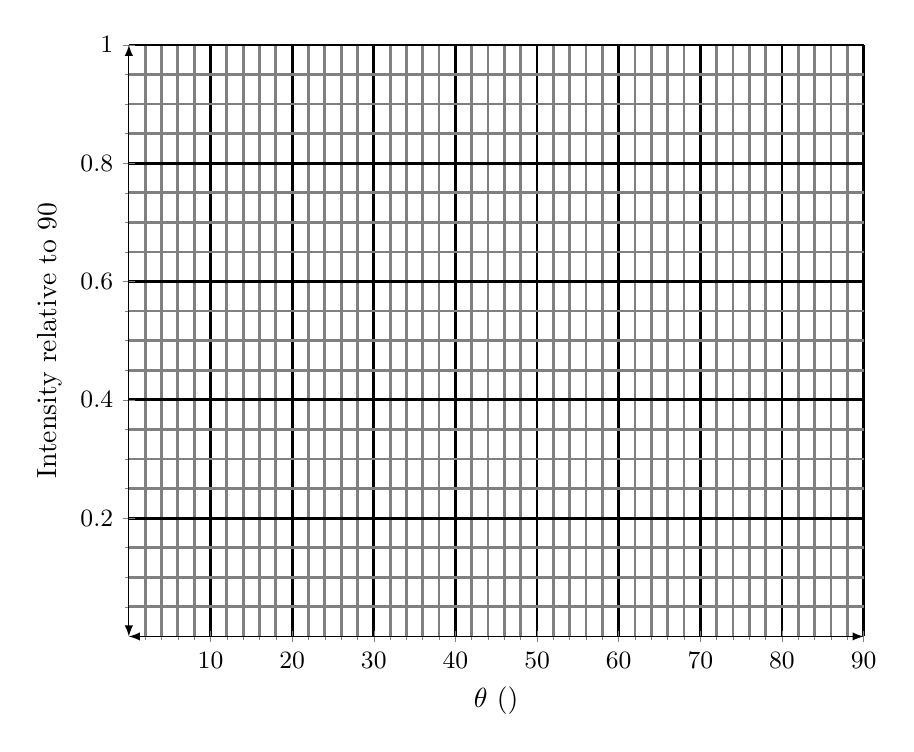
\begin{tikzpicture}
\begin{axis}[
	width=0.9\textwidth,
    height=0.75\textwidth,
    xmin=0,xmax=90,xtick={0,10,20,30,40,50,60,70,80,90},minor xtick={2,4,6,8,12,14,16,18,22,24,26,28,32,34,36,38,42,44,46,48,52,54,56,58,62,64,66,68,72,74,76,78,82,84,86,88},
    ymin=0,ymax=1,ytick={0,0.2,0.4,0.6,0.8,1.0},minor ytick={0.05,0.1,0.15,0.25,0.3,0.35,0.45,0.5,0.55,0.65,0.7,0.75,0.85,0.9,0.95},
    grid=both,
    grid style={line width=1pt, draw=gray!100},
    major grid style={line width=1pt, draw=black!100},
    axis lines=center,
    minor tick num=1,
    %enlargelimits={abs=0.5},
    axis line style={latex-latex},
    ticklabel style={font=\small},
    xlabel near ticks,
    ylabel near ticks,
    xlabel={$\theta$ (\si{\degree})},
    ylabel={Intensity relative to \SI{90}{\degree}}
]
\end{axis}
\end{tikzpicture}

\end{document}